\documentclass[../Article_Model_Parameters.tex]{subfiles}
\graphicspath{{\subfix{../Figures/}}}
\begin{document}
	
	\label{CH: Results}

    The parameter estimation problem was solved by fitting the process model to the dataset given in the Table \ref{tab: Yield_data}. Each time-series was fitted to the model separately. As a result of fitting, the following parameters were obtained:

    \begin{itemize}
        \item Partition coefficient:\qquad\quad\qquad$k_m$
        \item Internal Diffusion coefficient: \quad$D_i$
        \item Axial Diffusion coefficient: \qquad$D_e^M$
        \item Standard Deviation: \qquad\qquad\quad$\sigma$
    \end{itemize}

    Moreover, the initial state estimation was performed together with parameter estimation. The concentration of solute in the solid phase is assumed to be constant and uniformly distributed. On the other hand, the solute concentration in the fluid phase should not follow the same assumption as the solid phase. During the preparation period the solute diffuses to the fluid phase in contact with the solid particles. Later, the solute in the fluid phase is partially moved (if the pressure increase in the system, the pump cause the movement of the fluid, even if the outlet valve is closed) along the extractor. As a result, the distribution of solutes mass in the fluid phase is assumed to not be uniform. Some conclusions can be drawn from the analysis of the initial part of each yield curve. It can be noticed that each curve at the beginning has a curvature, which is not linear. In a general sense, it can be said that a quadratic function could approximate the initial part of each extraction curve. A function that, after integration, gives a quadratic-like result is a straight line. Based on that observation, the solute concentration in the fluid phase is assumed to be linearly distributed. The solute concentration is assumed to be zero at the outlet and reach the maximum at the beginning of the fixed bed. The details on the calculation are given in appendix \ref{CH: IC_BC}. The linear distribution can be defined if the total mass of solute $m_{total}$ and partition coefficient $\tau$ are know.
    
    Due to initial state estimation, two additional parameters are fitted.

    \begin{itemize}
        \item Total mass of solute: \qquad\qquad\quad$m_{total}$
        \item Partition coefficient: \qquad\qquad\quad$\tau$
    \end{itemize}

	To ensure that parameters found by the optimizer do not reach unrealistic values, an additional set of inequality constraints is introduced. The lower and upper bounds for each parameter are given in Table \ref{tab:Constraints}. The same Table contains the initial guesses for the optimizer. To ensure that the solution is a global solution multiple initial points have been tested.

	\begin{table}[!h]
		\centering
		\adjustbox{max width=\columnwidth}{%
		\begin{tabular}{ lcccccc }
			\hline 
			Parameter		&$k_m$ 	& $D_i$ 	& $D_e^M$ 	& $m_{total}$	& $\tau$ 	& $\sigma$ \\  \hline
			Lower bound		&0	  	& 0 	  	& 0 		& 76 		 	& 0 	   	& 0 \\ 
			Upper bound		&1 		& $+\infty$ & $+\infty$	& 100 			& 1 		& $+\infty$ \\ 
			Initial guess	&1	  	& 3 	  	& 1 		& 77 		 	& 0.65 	   	& 0.1 \\  \hline
		\end{tabular} }
	\caption{Constraints of the parameter estimation problem}
	\label{tab:Constraints}
	\end{table}

%	The parameter estimation problem requires an initial guess as an input to an optimization problem. To ensure that the solution is a global solution multiple initial points have been tested. The initial guesses for the parameter estimation problem are given in Table \ref{tab:InitialGuess}
	
%	\begin{table}[!h]
%		\centering
%		\adjustbox{max width=\columnwidth}{%
%		\begin{tabular}{ lcccccc } 
%			\hline
%			Parameter		&$k_m$ 	& $D_i$ 	& $D_e^M$ 	& $m_{total}$	& $\tau$ 	& $\sigma$ \\  \hline
%			Initial guess	&1	  	& 3 	  	& 1 		& 77 		 	& 0.65 	   	& 0.1 \\  \hline
%		\end{tabular} }
%		\caption{Constraints of the parameter estimation problem}
%		\label{tab:InitialGuess}
%	\end{table}
	
	The figure \ref{fig: estimation_results} show yield curves for each of experiments. The blue dots indicate the data point obtained as a measurement from the laboratory experiments. The black curve represents the yield curve obtained from the initial guess of the parameters. The blue curve correspond to yield curve obtained as a solution of the optimization problem. The curves on the left hand-side of the Figure \ref{fig: estimation_results}, are the cumulative yield curves, which represents the cumulative amount of the oil collected during each experiment. The Figures on the right hand-side, represent the derivative of the cumulative yield curves. As explained in the chapter \ref{CH: Parameter_estimation}, the derivatives of the cumulative measurements are independent on the previous measurement and should be used for the parameter estimation.

	\begin{table}[!h]
		\centering
		\adjustbox{max width=\columnwidth}{%
			\csvautobooktabular{Figures/Results_estimation/estimation.csv} }
		\caption{Parameter estimation results}
		\label{tab: Estimation_results}
	\end{table}

	The results of the parameter estimation can be found in Table \ref{tab: Estimation_results}. As can be noticed, the optimizer found that the partition factor should be as high as possible and moved values of $k_m$ for each experiment to unity, which was chosen as the upper bound.
		
	Values of the internal diffusion coefficients are distinguished for each experiment, with an increasing trend with respect to the fluid density. The order of magnitude of $D_i$ obtained from the optimization is similar to values found by other researchers. \citet{Reverchon1996} performed the parameter estimation for the extraction process of sage oil from seeds and reported $D_i \approx 6e-13$.
	
	The axial diffusion coefficient obtained from the optimizer seems to be quite high if compared to the internal diffusion coefficients. Nevertheless, the values of $D_e^M$ have similar order of magnitude as reported in literature, for example \citet{ReisVasco2000}. The relatively high values of the axial diffusion coefficients might be justified by taking into account low values of flow rate used in all the experiments.
	
	As the total amount of the oil present in the system is unknown, and as such it has been obtained from the optimizer. Given the dataset and the process model, the optimizer found that all most all the oil was extracted out of the seeds and that the best fit is obtained if the total mass of the oil reach a lower bound equal to 76 g.
	
	As explained above, and in Appendix \ref{CH: IC_BC}, the linear distribution of can be fully determined if the parameter $\tau$ is known. The split ratio for experiments conducted at $40 ^\circ C$ / 300 bar and $50 ^\circ C$ / 300 bar are similar to each other and close to 0.64. The experiments performed at $40 ^\circ C$ / 200 bar and $50 ^\circ C$ / 200 bar have $\tau$ equals to $0.69$ and $0.74$, respectively. 
	
	The noise present in each dataset is quantified by parameter $\sigma$. It can be observed dataset obtained at $40 ^\circ C$ / 200 bar, $50 ^\circ C$ / 200 bar and $40 ^\circ C$ / 300 bar have similar value of $\sigma\approx0.34$. The visual investigation of the dataset obtained at $50 ^\circ C$ / 300 bar allow to explain higher value of $\sigma$ for this dataset. This dataset have higher deviation of the data points from the simulated curve.
	
		\begin{figure}[!h]
		\centering
		\begin{subfigure}[b]{\columnwidth}
			\centering
			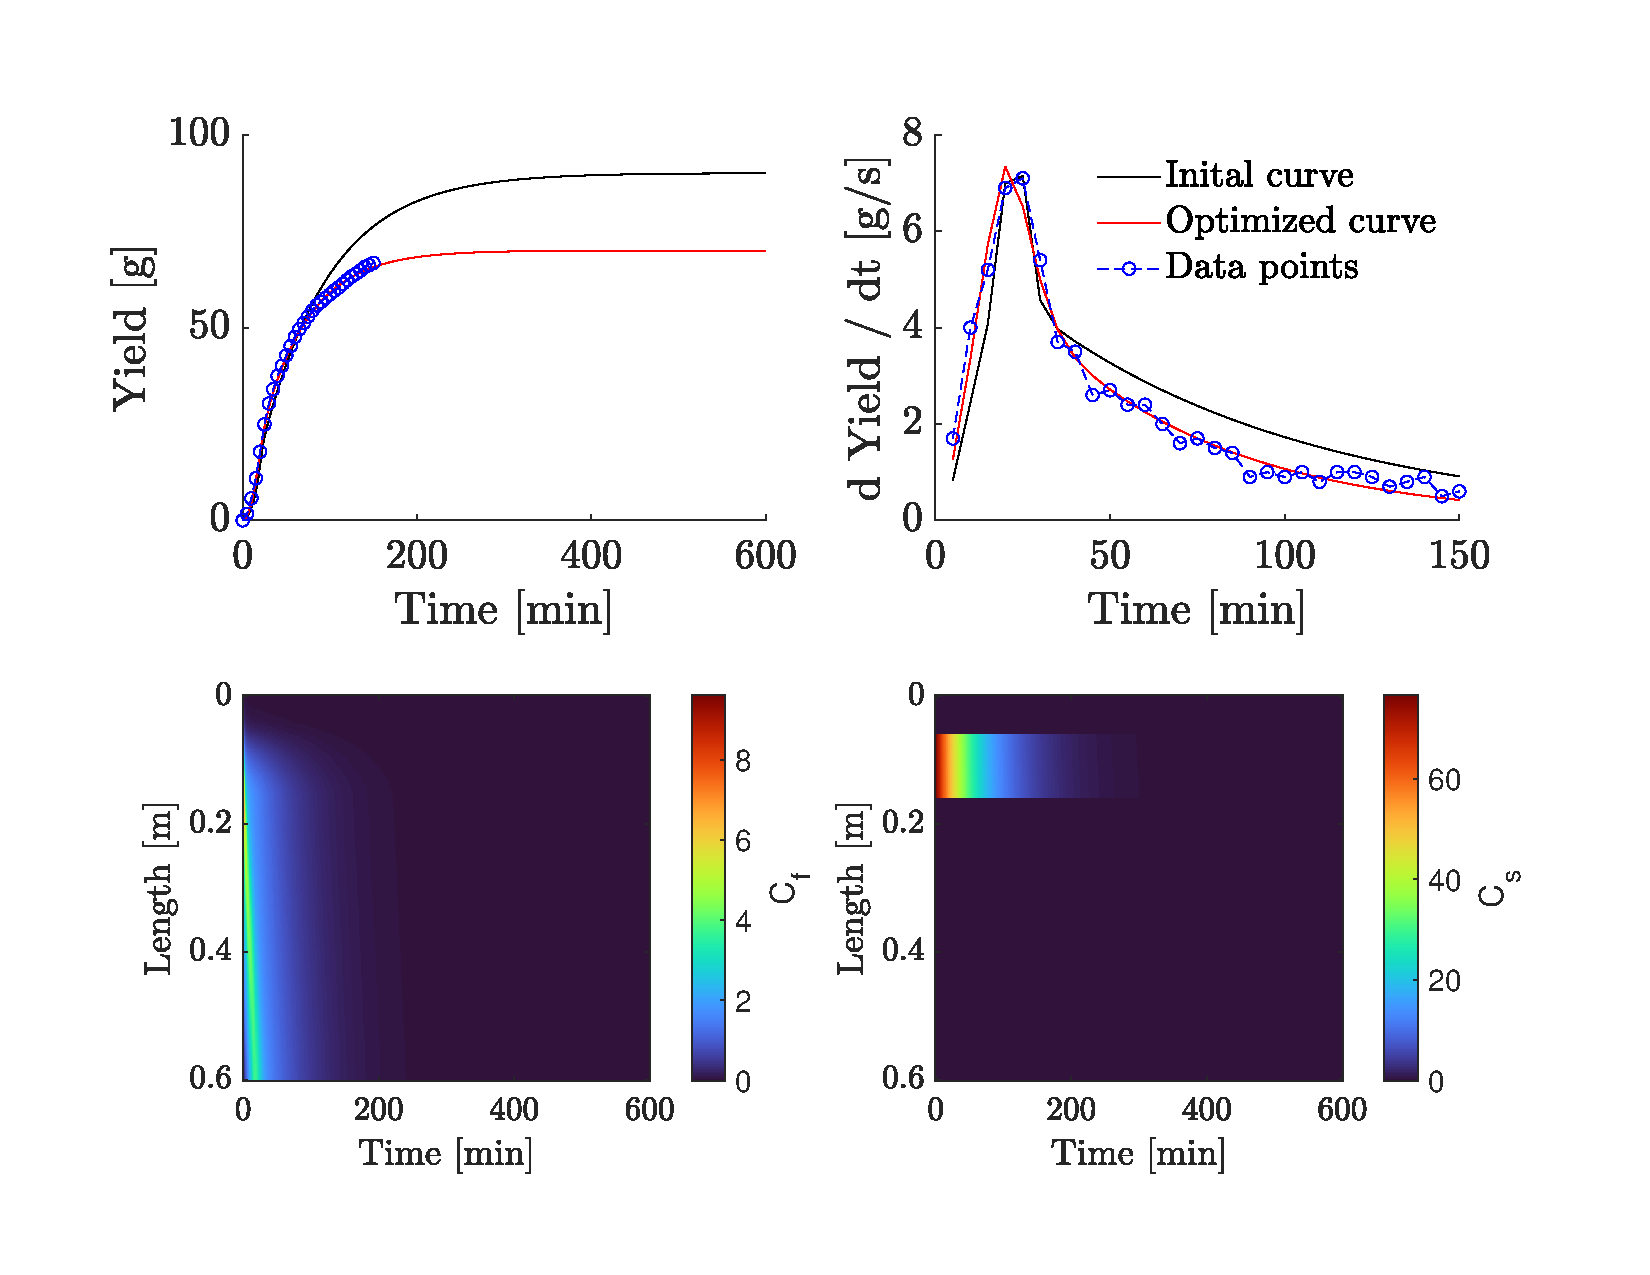
\includegraphics[trim = 3cm 11cm 2.5cm 2.1cm,clip,width=\textwidth]{/Results_estimation/Fitting_LUKE_T40_P200.pdf}
			\caption{Experiment at $40^\circ C$ and $200$ bar}
		\end{subfigure}
		\begin{subfigure}[b]{\columnwidth}
			\centering
			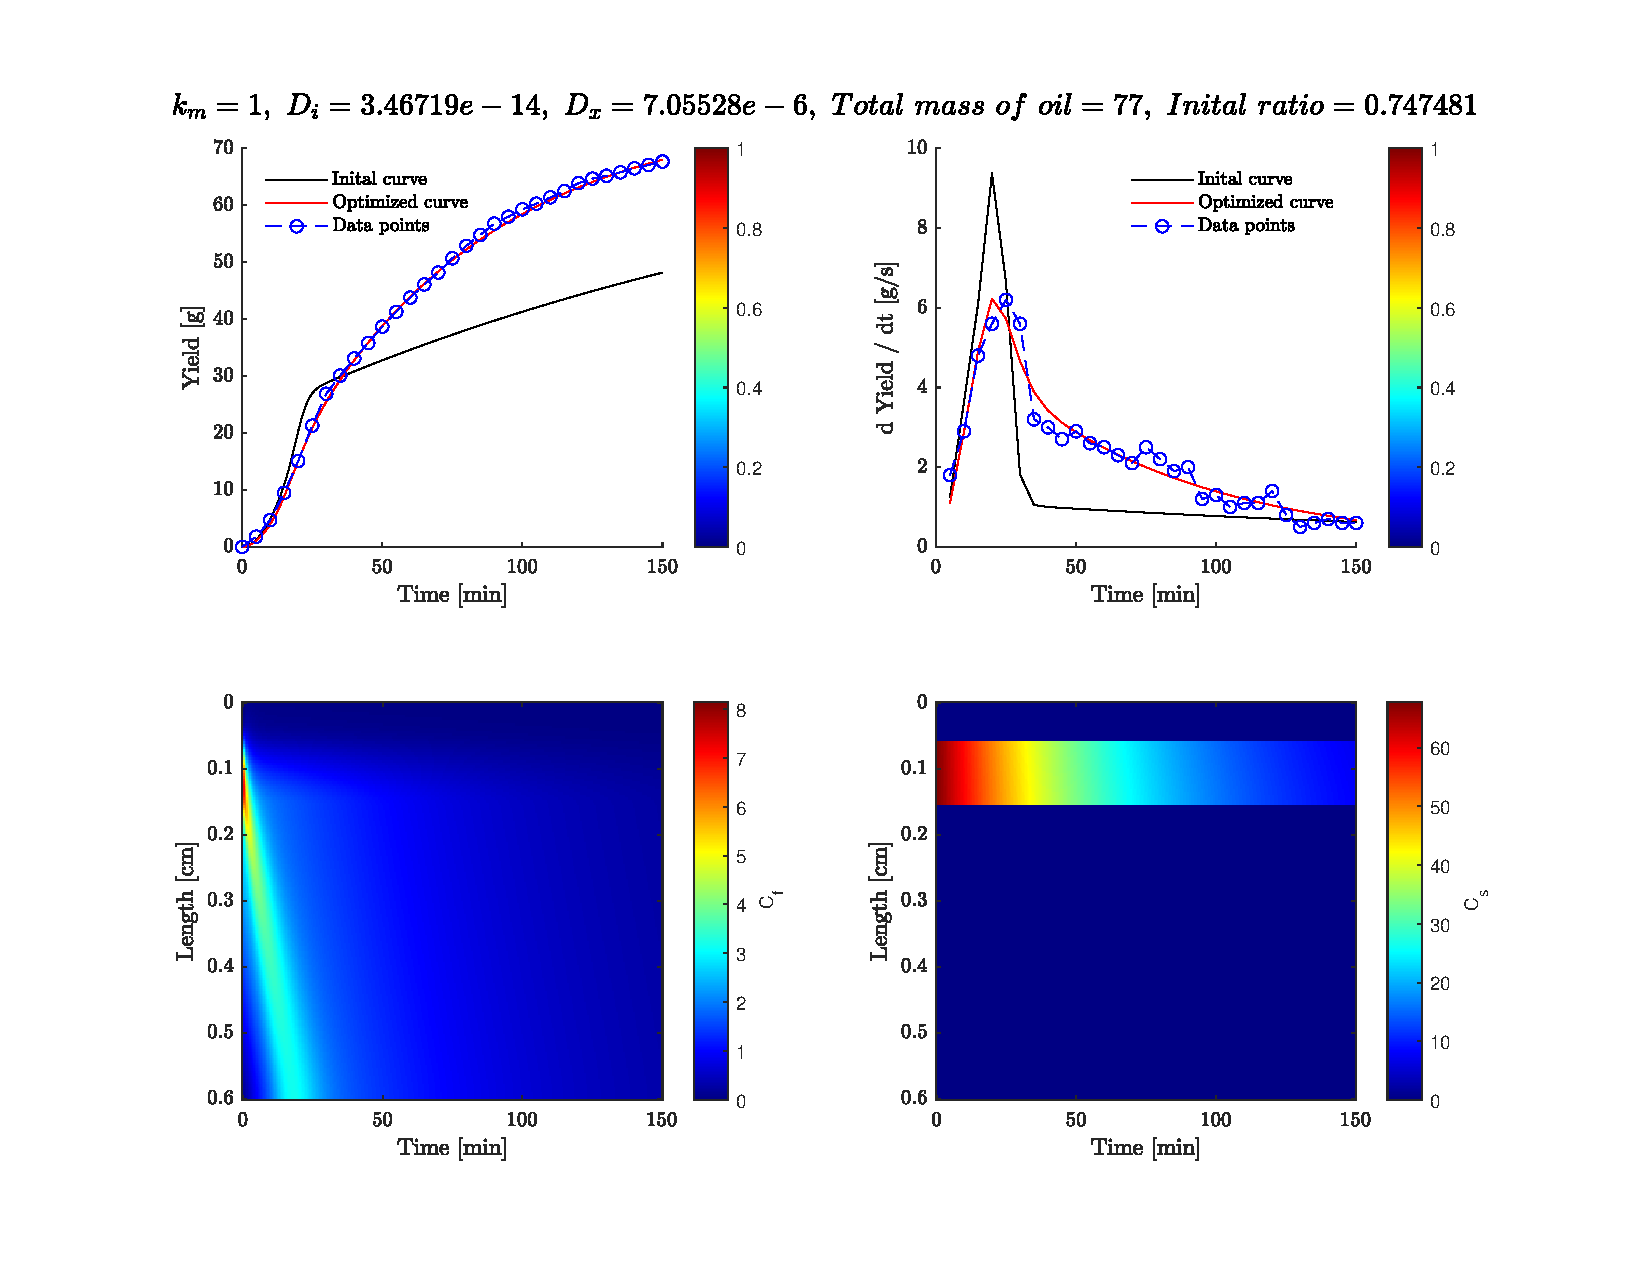
\includegraphics[trim = 3cm 11cm 2.5cm 2.1cm,clip,width=\textwidth]{/Results_estimation/Fitting_LUKE_T50_P200.pdf}
			\caption{Experiment at $50^\circ C$ and $200$ bar}
		\end{subfigure}
		\begin{subfigure}[b]{\columnwidth}
			\centering
			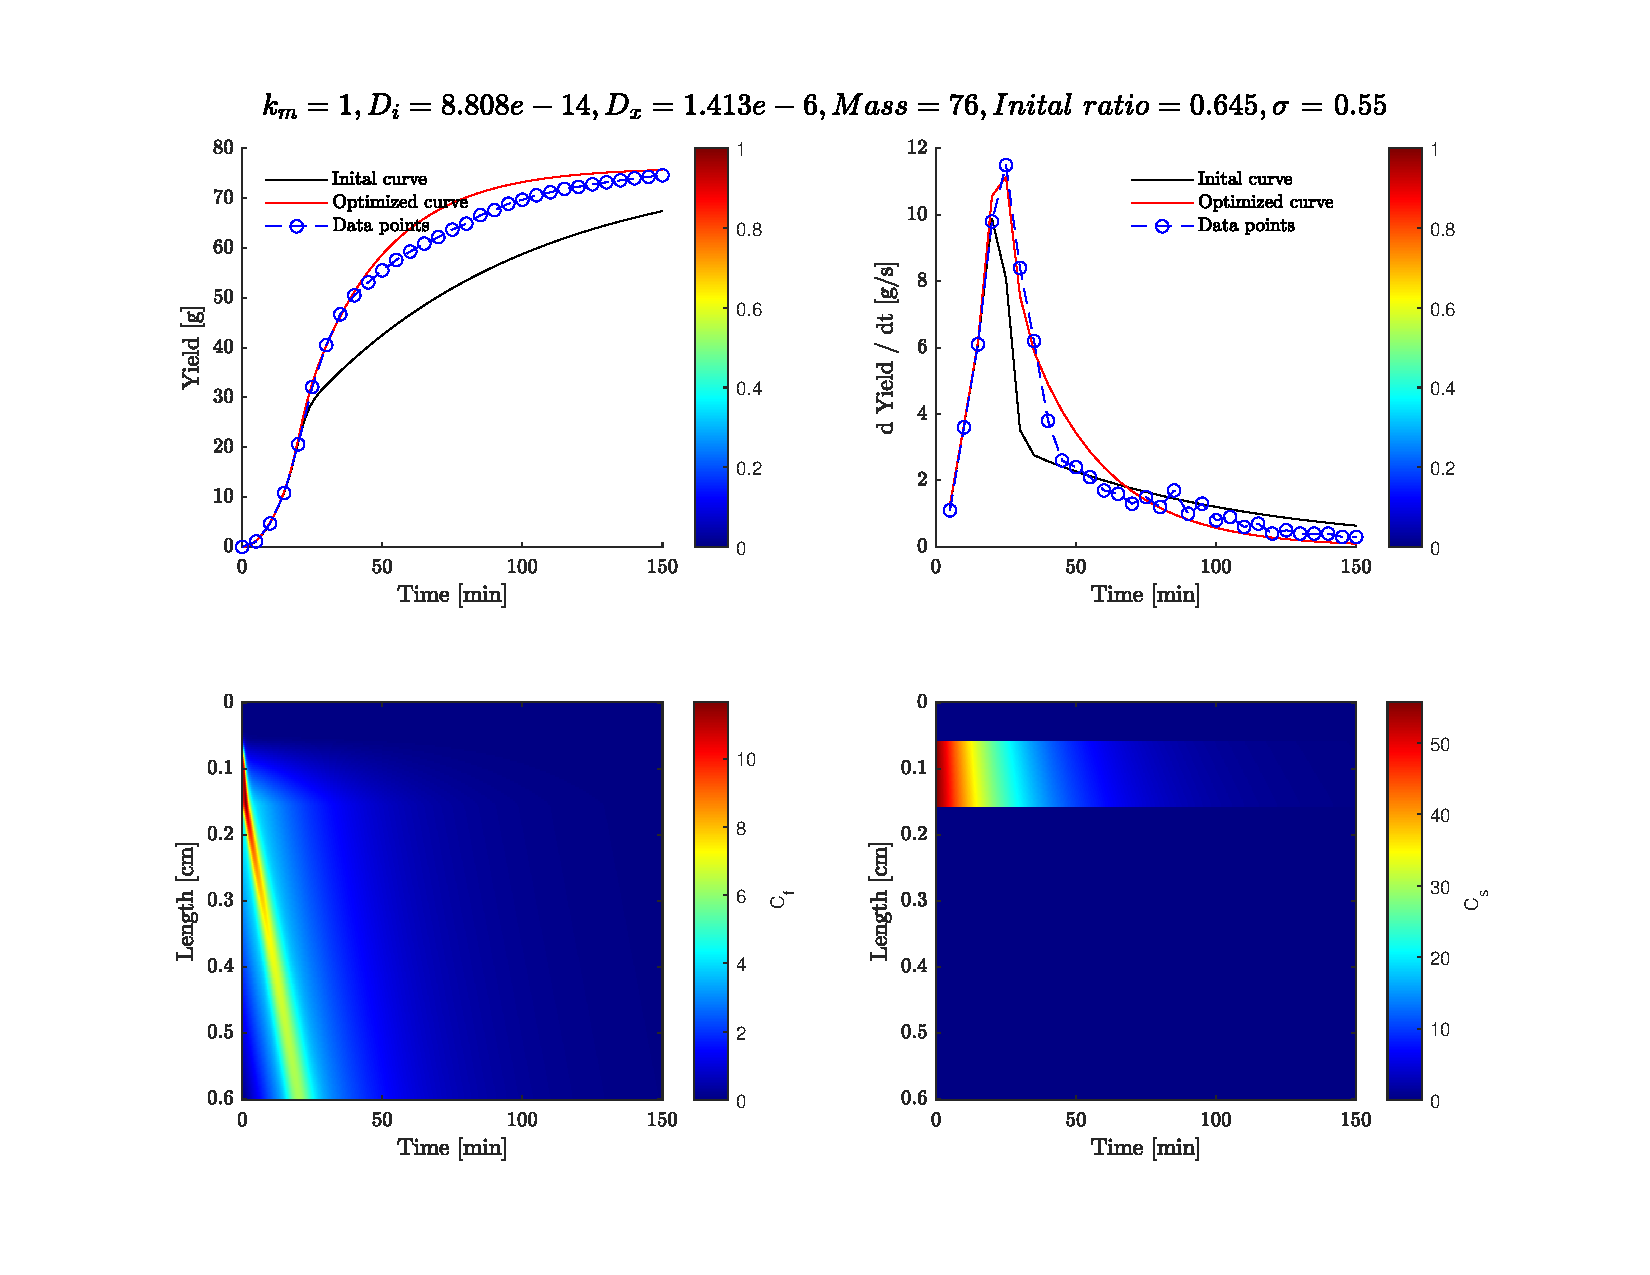
\includegraphics[trim = 3cm 11cm 2.5cm 2.1cm,clip,width=\textwidth]{/Results_estimation/Fitting_LUKE_T40_P300_org.pdf}
			\caption{Experiment at $40^\circ C$ and $300$ bar}
		\end{subfigure}
		\begin{subfigure}[b]{\columnwidth}
			\centering
			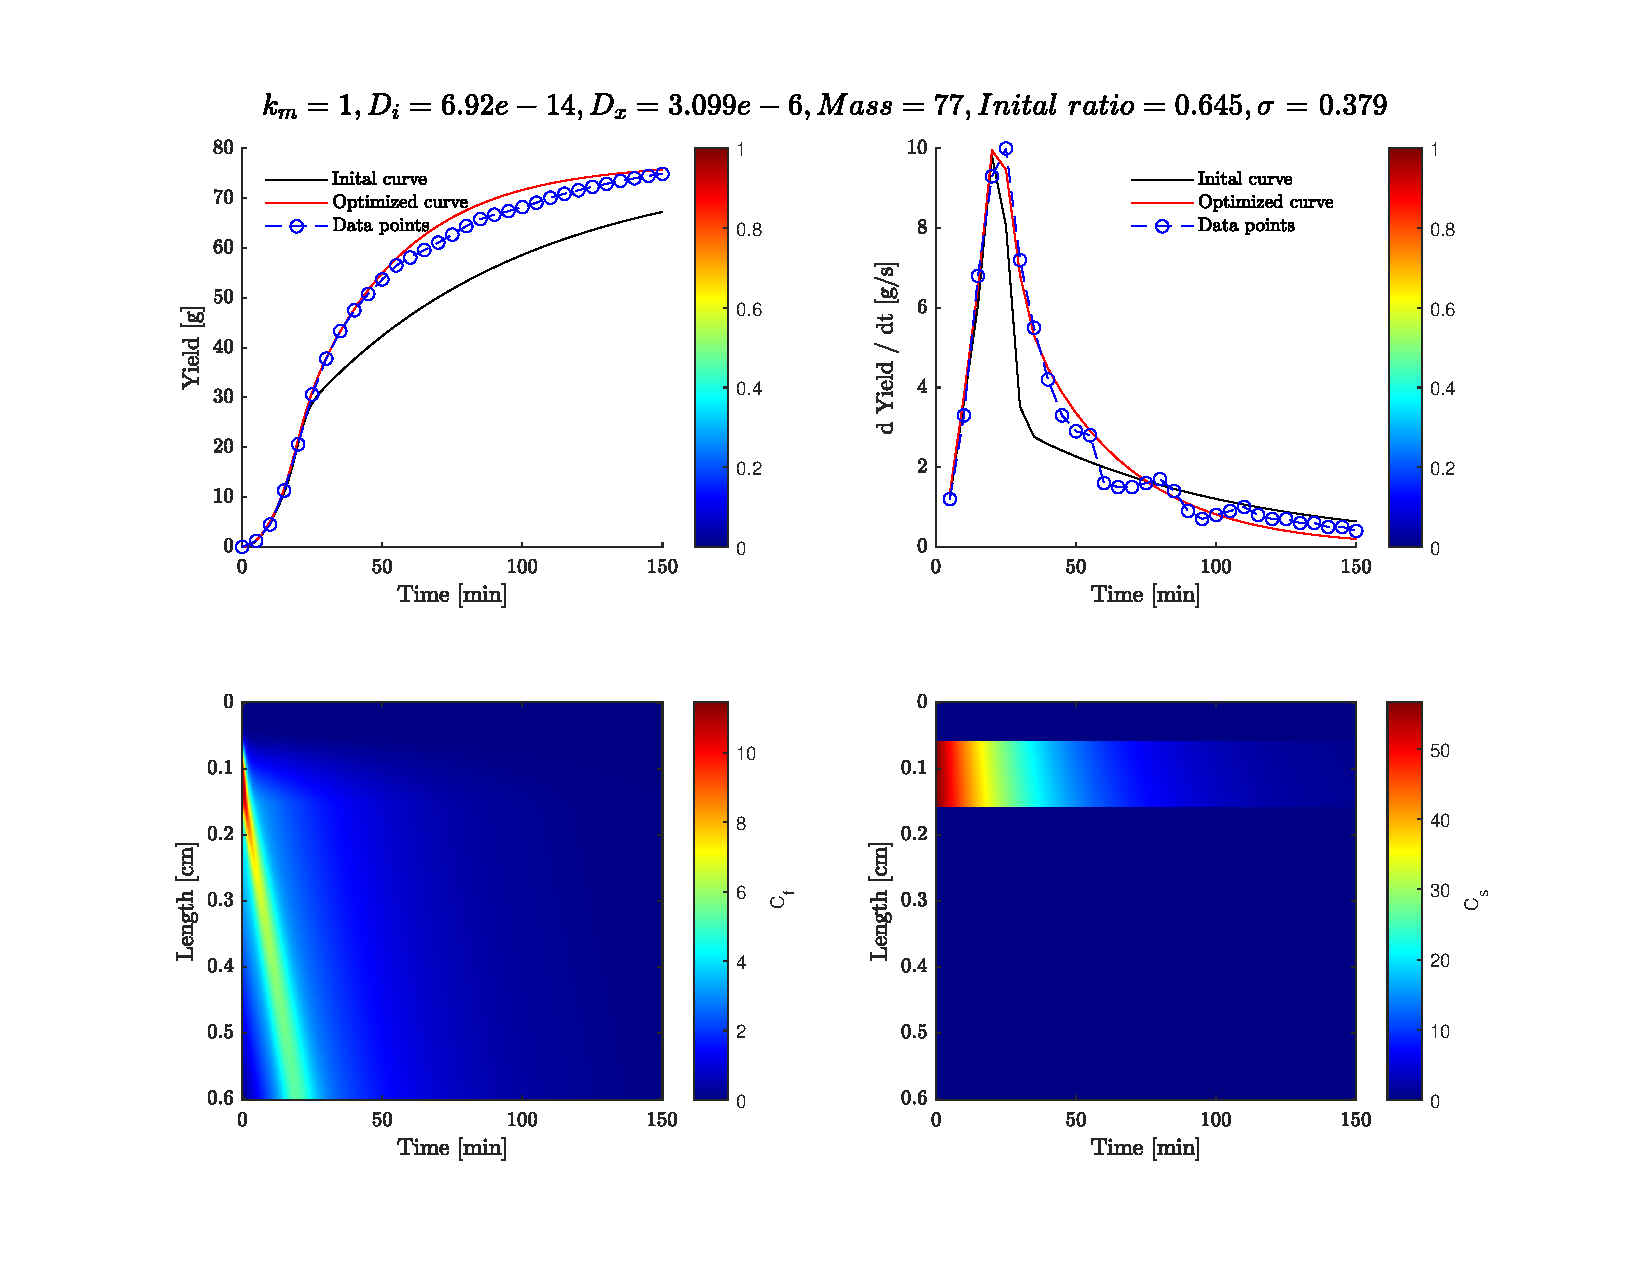
\includegraphics[trim = 3cm 11cm 2.5cm 2.1cm,clip,width=\textwidth]{/Results_estimation/Fitting_LUKE_T50_P300_org.pdf}
			\caption{Experiment at $50^\circ C$ and $300$ bar}
		\end{subfigure}
		\caption{Results of parameter fitting, with estimation of the initial state}
		\label{fig: estimation_results}
	\end{figure}

	The results obtained from the parameter estimation are used to develop a generalized process model. This model expresses the parameters $D_i$ and $D_e^M$ as functions of the operating conditions, such as temperature (T), pressure (P), and flow rate (F). Since the experiments were performed under varying temperature and pressure, the influence of these variables is taken into account. To simplify the problem, the correlations are written as functions of fluid density rather than temperature and pressure.
	
	While the experimental procedure and device can affect $\tau$ and $\sigma$, these parameters are not further considered. They are used only to define the initial conditions and are not included in the process model. Additionally, since the optimizer found that $k_m$ and $m_{total}$ have the same value, they are assumed to be constants and not considered further.
	
	The other two parameters ($D_i$ and $D_e^M$) are subject to regression to obtain correlations in terms of density. Figure \ref{fig:Regression} shows the first- and second-order polynomials used to fit $D_i$ and $D_e^M$ as a function of fluid density. Interestingly, these two parameters exhibit opposite behavior.

	\begin{figure}[!h]
	\centering
	\begin{subfigure}[b]{\columnwidth}
		\centering
		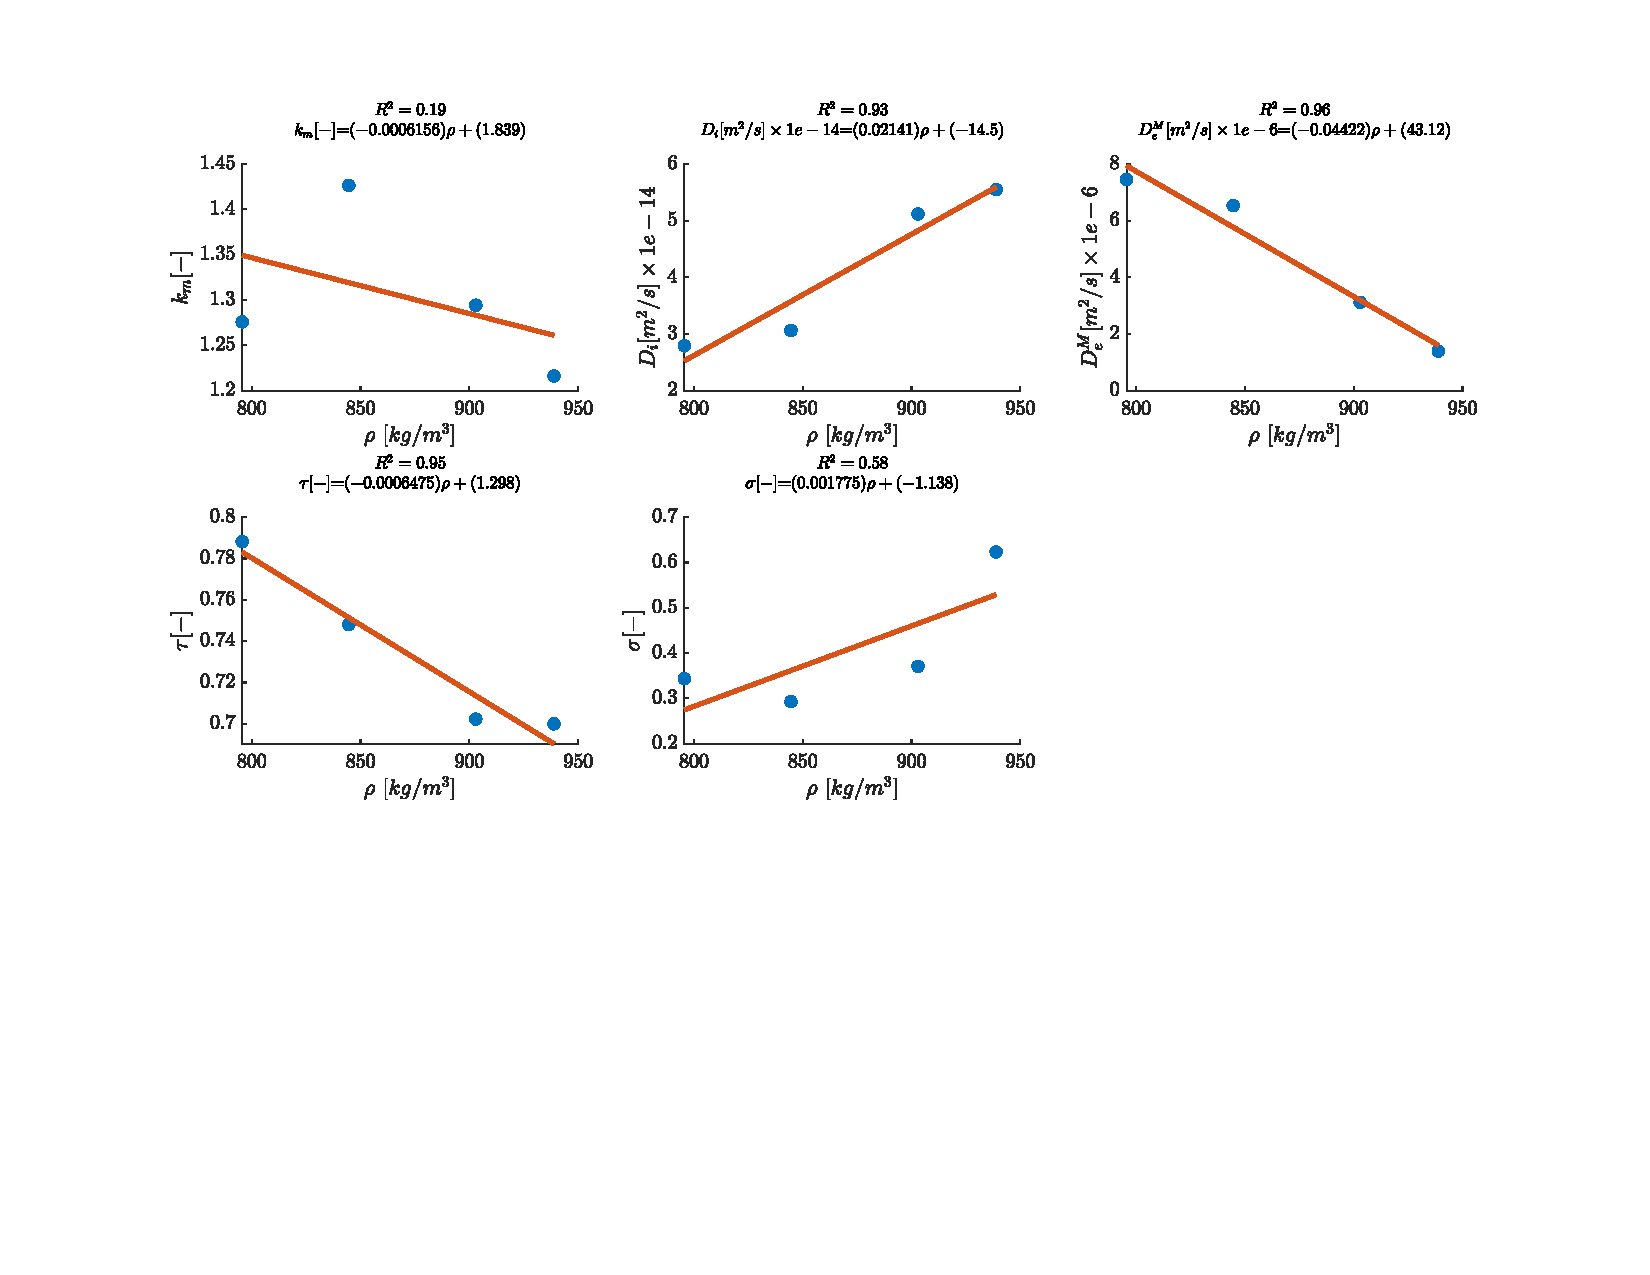
\includegraphics[trim = 10.5cm 11cm 2.5cm 1cm,clip,width=\textwidth]{/Results_estimation/Trend_Lines_order_1.pdf}
		\caption{First order polynomial regression of fitted parameters as a function of fluid density $\rho_f$}
		\label{fig:Regression_1}
	\end{subfigure}
	\begin{subfigure}[b]{\columnwidth}
		\centering
		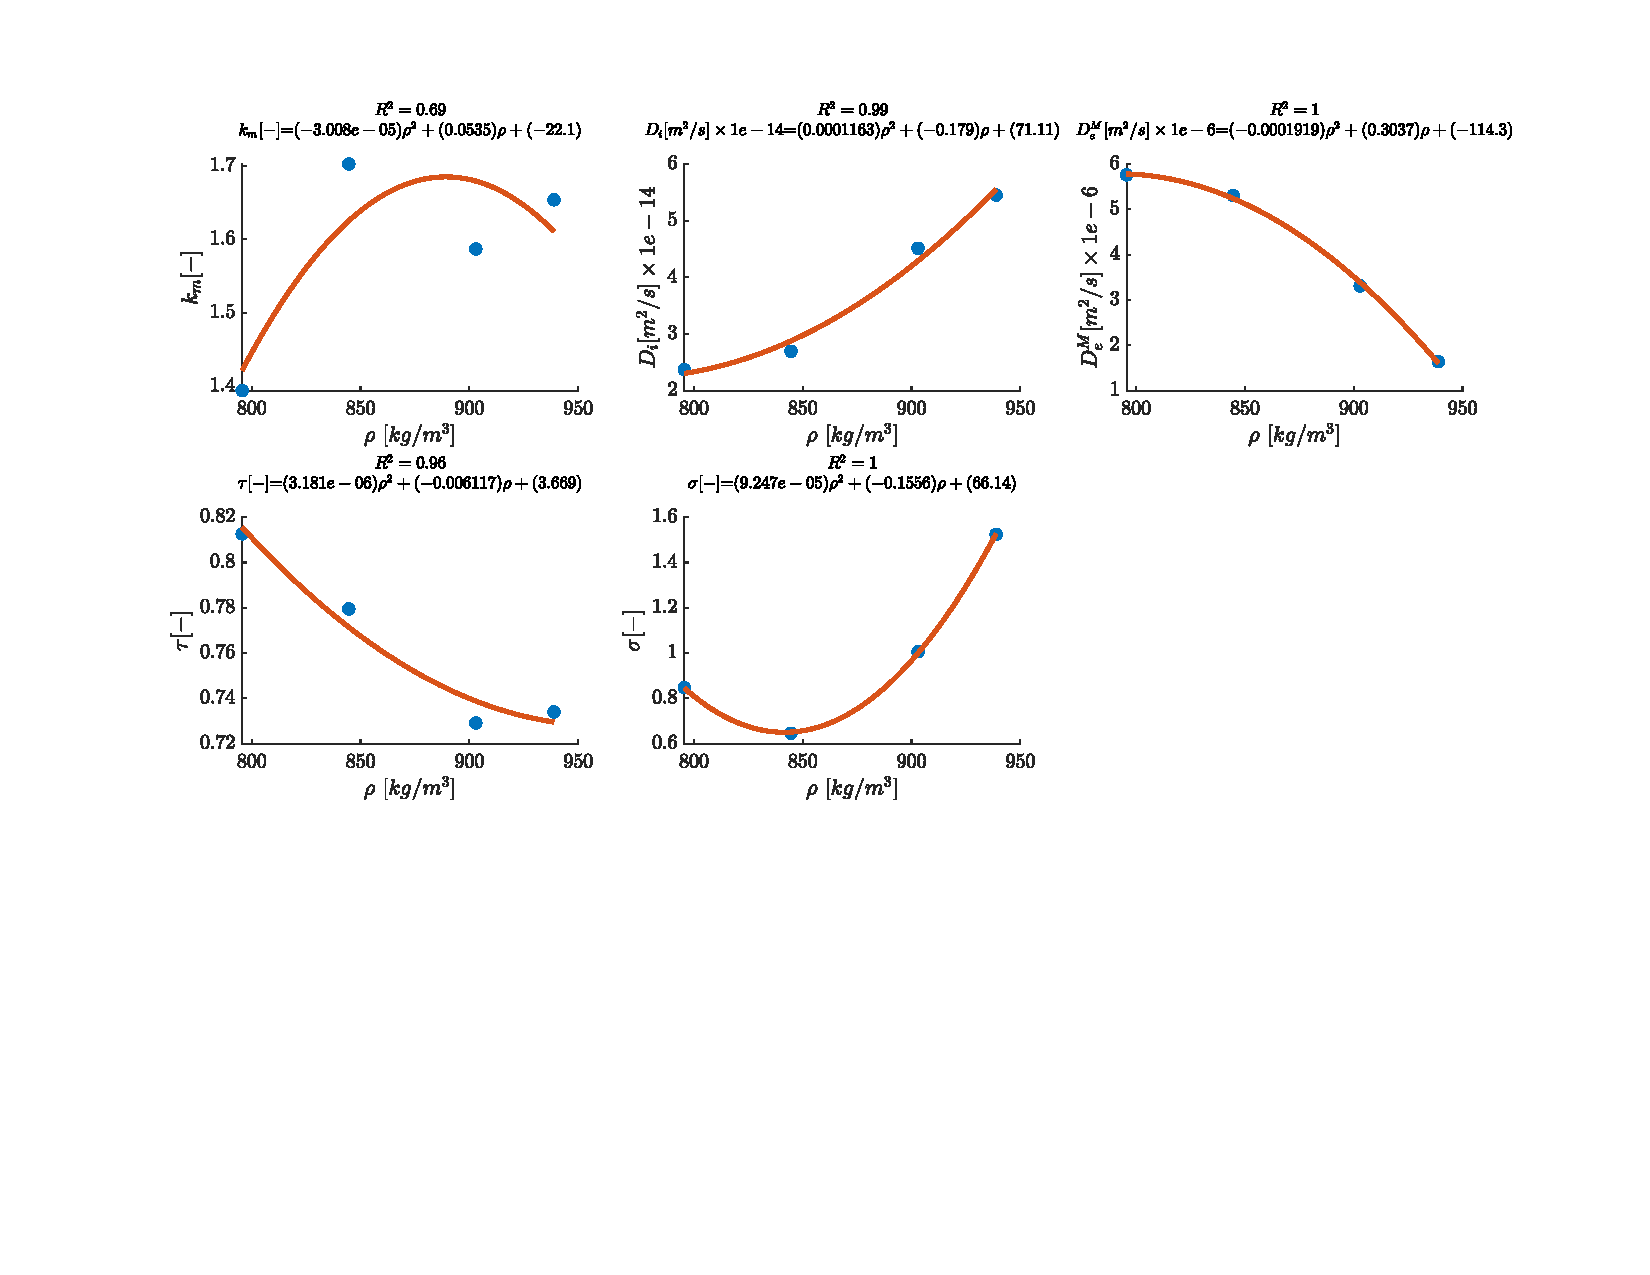
\includegraphics[trim = 10.5cm 11cm 2.5cm 1cm,clip,width=\textwidth]{/Results_estimation/Trend_Lines_order_2.pdf}
		\caption{Second order polynomial regression of fitted parameters as a function of fluid density $\rho_f$}
		\label{fig:Regression_2}
	\end{subfigure}
	\caption{Results of parameter fitting, with estimation of the initial state} 
	\label{fig:Regression}
	\end{figure}

	The results of the linear regression applied to $D_i$ and $D_e^M$ are presented in Figure \ref{fig:Regression_1}. It can be observed that the internal diffusion coefficient increases with increasing fluid density, while the axial diffusion coefficient decreases.
	
	The increase in the density of the supercritical fluid can lead to an increase in the solubility of the solute and, consequently, an increase in the concentration gradient. This increased concentration gradient drives the solute to diffuse more rapidly through the matrix of the solid particles, resulting in an increase in the internal mass transfer coefficient. However, the effect of increased solubility on the internal mass transfer coefficient is greater than the resistance coming from higher density, resulting in an overall increase in the internal mass transfer coefficient with density.
	
	The behaviour of the axial diffusion coefficient can be explained through Graham’s Law of Diffusion, which states that the rate of diffusion of a molecule is inversely proportional to the square root of its density under given conditions of temperature and pressure. This means that denser media slow down the axial diffusion rate of molecules. 
	
	{\color{red}IDEAL I SHOULD SUPPORT THIS EXPLANATION WITH SOME REFERENCES}
	
	Figure \ref{fig:Regression_1} show the result of fitting a second-order polynomial in density space. It can be observed that the fit obtained from quadratic functions seems to be represent both dataset better. 
	
	
\end{document}